
\section{平坦性的局部判别法}

对于\trNoether{}局部环，\mbox{定理~24.3.1} 的理想论判别法有一个大为改进的版本：我们只须检验\emph{一个}理想——极大理想。

\textbf{24.6.1. \trhTheorem（平坦性的局部判别法）。}\ ——\ \emph{设 $(B,\mathfrak{n})\to(A,\mathfrak{m})$ 是\trNoether{}局部环之间的一个局部态射（\S7.3.1），而 $M$ 是有限生成的 $A$-\trModule。则 $M$ 是 $B$-平坦的，当且仅当 $\mathrm{Tor}^B_1(M,B/\mathfrak{n})=0$。}

这是一个奇迹：整个 $\Spec B$ 上的平坦性，竟由闭点处发生的事情决定。

\mbox{定理~24.6.1} 的一个特殊情形我们已经见过：若 $(B,\mathfrak{n})\to(A,\mathfrak{m})$ 是\trIsomorphism，则它是\mbox{定理~24.3.5} 的直接推论。

下面的证明归于 Ogus，[OB]。为了凸显证明何以奏效，我们暂且给出一个（其实用不上的）定义。

\textbf{24.6.2.}\ \emph{\trhDefinition。}\quad 设 $F\colon\mathscr{B}\to\mathscr{A}$ 是\trAbelianCategory{}之间的一个\trAdditiveFunctor。仅在本节中，我们说 $F$ 是\textbf{\trHalfExact}（half-exact）的，如果对 $\mathscr{B}$ 中每个\trShortExactSequence{} $0\to M'\to M\to M''\to 0$，$FM'\to FM\to FM''$ 都在 $\mathscr{A}$ 中正合。左正合函子、右正合函子，以及二者的\trDerivedFunctor，都是\trHalfExact{}的例子。

\textbf{24.6.3. \trhTheorem（\trHalfExact{}函子的\trNakayama{}引理）。}\ ——\ \emph{设 $(B,\mathfrak{n})\to(A,\mathfrak{m})$ 是\trNoether{}局部环之间的一个局部态射，而加性函子 $T\colon\mathit{f.g.Mod}_B\to\mathit{f.g.Mod}_A$ 是 $B$-线性的且\trHalfExact{}。若 $T(B/\mathfrak{n})=0$，则对一切有限生成的 $B$-\trModule{} $N$ 都有 $T(N)=0$（也就是说，$T$ 是零函子）。}

\emph{证明。}\quad 我们要使用 $A$ 的\trNakayama{}引理，取其如下形式：若 $M\in\mathit{f.g.Mod}_A$，$a\in\mathfrak{m}$，而映射 $M\xrightarrow{\ \times a\ }M$ 是满射，则 $M=0$。（到现在你应该已经能够看出，这是 \S8.2.7 中\trNakayama{}引理的众多版本之一。）

为方便起见，令 $k=B/\mathfrak{n}$。我们希望证明：对一切 $M\in\mathit{f.g.Mod}_B$ 都有 $T(M)=0$。若不然，由 $M$ 的诺特性，存在极大的 $M'\subset M$ 使得 $T(M/M')\ne 0$。取一个这样的极大 $M'$。

令 $N=M/M'$，于是 $T(N)\ne 0$，但对 $N$ 的每个非平凡商 $N''$ 都有 $T(N'')=0$。于是我们希望证明的是：若 $N\in\mathit{f.g.Mod}_B$，且对 $N$ 的每个真商 $N''$ 都有 $T(N'')=0$，则 $T(N)=0$。

令 $I=\mathrm{Ann}(N)=\{b\in B: bN=0\}$。若 $I=B$，则 $N=0$，从而 $T(N)=0$。若 $I=\mathfrak{n}$，则 $N=(B/\mathfrak{n})^{\oplus m}$（$N$ 诺特蕴含 $m$ 有限），从而 $T(N)=T(B/\mathfrak{n})^{\oplus m}=0$。否则，存在 $b\in\mathfrak{n}\setminus I$。

考虑短正合列
\[
0 \longrightarrow bN \longrightarrow N \longrightarrow N/bN \longrightarrow 0.
\]
由于 $bN\ne 0$，$N/bN$ 是 $N$ 的一个非平凡商，故 $T(N/bN)=0$。由 $T$ 的\trHalfExact{}性，既然 $T(N)\ne 0$，便有 $T(bN)\ne 0$。

接下来，考虑短正合列
\[
0 \longrightarrow \ker\bigl(N \xrightarrow{\ \times b\ } N\bigr) \longrightarrow N \xrightarrow{\ \times b\ } bN \longrightarrow 0.
\]
由于 $T(bN)\ne 0$，$bN$ 并\emph{不是} $N$ 的非平凡商，故 $\ker(N\xrightarrow{\ \times b\ }N)=0$。于是我们有第三个短正合列
\[
0 \longrightarrow N \xrightarrow{\ \times b\ } N \longrightarrow N/bN \longrightarrow 0,
\]
由此得
\[
T(N) \xrightarrow{\ \times T(b)\ } T(N) \longrightarrow T(N/bN) = 0
\]
正合。（这里我们利用 $T$ 的 $B$-线性，把映射 $T(N)\to T(N)$ 认同为乘以 $T(b)\in\mathfrak{m}$。）于是由 $A$ 的\trNakayama{}引理，$T(N)=0$，与 $T(N)\ne 0$ 矛盾。\hfill$\square$

\textbf{24.6.4.}\ \emph{\mbox{定理~24.6.1} 的证明。}\quad 设 $M$ 是有限生成的 $A$-\trModule。一个方向是容易的：若 $M$ 在 $B$ 上平坦，则由 $\mathrm{Tor}$ 判别法（\mbox{练习~23.1.C}），$\mathrm{Tor}^B_1(M,B/\mathfrak{n})=0$。

较难的方向：现设 $\mathrm{Tor}^B_1(M,B/\mathfrak{n})=0$。定义 $T\colon\mathit{f.g.Mod}_B\to\mathit{f.g.Mod}_A$，$N\mapsto\mathrm{Tor}^B_1(M,N)$。则 $T$ 是 $A$-线性的（你能看出为什么吗？）且\trHalfExact{}。由\trHalfExact{}函子的\trNakayama{}引理，$T(B/\mathfrak{n})=0$ 蕴含：对一切有限生成的 $B$-\trModule{}都有 $T(N)=0$，特别地，对一切 $B/I$ 如此；再由平坦性的理想论判别法（\mbox{定理~24.3.1}），即见 $M$ 在 $B$ 上平坦。\hfill$\square$

\textbf{24.6.5. 平坦性的\trSlicing{}判别法。}\quad 局部判别法有一个有用的变体如下。设 $t\in\mathfrak{n}$ 是 $B$ 的一个\trNonZerodivisor（几何上说：这是靶上经过闭点的一个\trEffectiveCartierDivisor）。若 $M$ 在 $B$ 上平坦，则 $t$ 不是 $M$ 的\trZerodivisor（\mbox{观察~24.1.2}）。而且 $M/tM$ 是平坦的 $B/tB$-\trModule（平坦性与基变换交换，\mbox{练习~24.1.J}）。下面这条结果说，这组条件反过来刻画了平坦性——至少当 $M$ 有限生成（或稍再一般一些）时如此。

\textbf{24.6.6. \trhTheorem（平坦性在靶上的\trSlicing{}判别法，见图~\ref{fig:slicing-target-criterion}）。}\ ——\ \emph{设 $(B,\mathfrak{n})\to(A,\mathfrak{m})$ 是\trNoether{}局部环之间的一个局部态射，$M$ 是有限生成的 $A$-\trModule，而 $t\in\mathfrak{n}$ 在 $B$ 上不是\trZerodivisor。则 $M$ 是 $B$-平坦的，当且仅当}
\begin{itemize}
\item[（i）]\emph{$t$ 不是 $M$ 的\trZerodivisor，而且}
\item[（ii）]\emph{$M/tM$ 在 $B/(t)$ 上平坦。}
\end{itemize}

\begin{figure}[htbp]
\centering
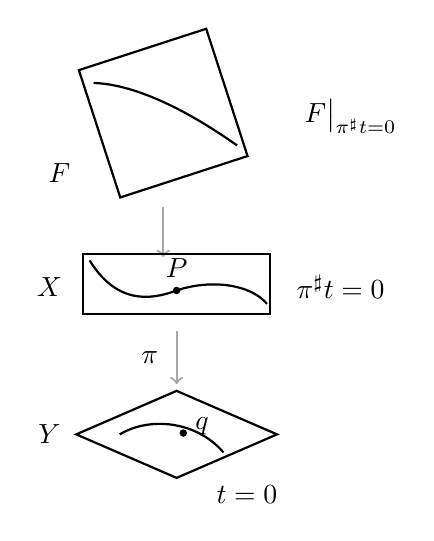
\begin{tikzpicture}[scale=0.85, line width=0.8pt]
  \begin{scope}[rotate around={18:(1.7,4.6)}]
    \draw (0.7,3.6) rectangle (2.7,5.6);
    \draw (0.85,5.35) .. controls (1.4,5.15) and (2.0,4.6) .. (2.6,3.8);
  \end{scope}
  \node at (0.15,3.7) {$\mathscr{F}$};
  \node at (4.5,4.55) {$\mathscr{F}\bigr|_{\pi^{\sharp}t=0}$};
  \draw[gray!70,->] (1.7,3.2) -- (1.7,2.45);
  \draw (0.5,1.6) rectangle (3.3,2.5);
  \draw (0.6,2.4) .. controls (1.0,1.75) and (1.5,1.8) .. (1.9,1.95)
        .. controls (2.4,2.12) and (3.0,2.05) .. (3.25,1.75);
  \fill (1.9,1.95) circle (1.6pt);
  \node at (1.9,2.28) {$P$};
  \node at (0.0,2.0) {$\mathscr{X}$};
  \node at (4.35,2.0) {$\pi^{\sharp}t=0$};
  \draw[gray!70,->] (1.9,1.35) -- (1.9,0.55);
  \node at (1.5,0.95) {$\pi$};
  \draw (1.9,0.45) -- (3.4,-0.2) -- (1.9,-0.85) -- (0.4,-0.2) -- cycle;
  \draw (1.05,-0.2) .. controls (1.5,0.07) and (2.2,0.0) .. (2.6,-0.47);
  \fill (2.0,-0.18) circle (1.6pt);
  \node at (2.28,-0.08) {$q$};
  \node at (0.0,-0.2) {$\mathscr{Y}$};
  \node at (2.95,-1.1) {$t=0$};
\end{tikzpicture}
\caption{平坦性在靶上的（充分必要的）\trSlicing{}判别法，\mbox{定理~24.6.6}。（依原书手绘图重绘。）}\label{fig:slicing-target-criterion}
\end{figure}

（关于其他性质的\trSlicing{}判别法，见\mbox{练习~13.2.C}、\mbox{定理~24.6.9} 与\mbox{定理~26.2.3}。）

为证此定理，我们先证一条引理，它还将用于证明\mbox{定理~24.6.14}。（注意：它对局部环或有限生成不作任何假设。）

\textbf{24.6.7. \trhLemma。}\ ——\ \emph{设 $I\subset B$ 是一个\trIdeal，$M$ 是一个 $B$-\trModule。又设（i）$\mathrm{Tor}^B_1(B/I,M)=0$，且（ii）$M/IM$ 在 $B/I$ 上平坦。则对每个包含 $I$ 的\trIdeal{} $J$ 都有 $\mathrm{Tor}^B_1(B/J,M)=0$。}

\emph{证明。}\quad 函子 $\otimes_B B/J$ 是函子 $\otimes_B B/I$ 与函子 $\otimes_{B/I}B/J$ 的复合。由\trGrothendieck{}函子复合谱序列（\S23.3.5），存在一个谱序列，其 $\Eto{p,q}{2}$ 项为 $\mathrm{Tor}^{B/I}_p\bigl(B/J,\mathrm{Tor}^B_q(B/I,M)\bigr)$，抵达 $\mathrm{Tor}^B_{p+q}(B/J,M)$。定理的假设保证
\[
\mathrm{Tor}^{B/I}_0\bigl(B/J,\mathrm{Tor}^B_1(B/I,M)\bigr)=0
\]
（由 (i)），以及
\[
\mathrm{Tor}^{B/I}_1\bigl(B/J,\mathrm{Tor}^B_0(B/I,M)\bigr)=\mathrm{Tor}^{B/I}_1(B/J,M/IM)=0
\]
（由 (ii)；这里对 $B/I$ 用了平坦性的理想论判别法，\mbox{定理~24.3.1}）。于是 $\mathrm{Tor}^B_1(B/J,M)=0$，此即所欲证。（不借谱序列这台机器，本证明也可以干脆用手工完成。）\hfill$\square$

\textbf{24.6.8.}\ \emph{平坦性在靶上的\trSlicing{}判别法（\mbox{定理~24.6.6}）的证明。}\quad 于是，在前一条引理中取 $I=(t)$、$J=\mathfrak{n}$，并利用\mbox{练习~24.2.A} 所给的 $\mathrm{Tor}^B_1(B/tB,M)=\ker(M\xrightarrow{\ \times t\ }M)$——由假设它为零——\mbox{定理~24.6.6} 便随之而得。\hfill$\square$

\textbf{24.6.A.（练习）}\quad 用\trSlicing{}判别法给出\mbox{练习~24.3.I}（$\mathbb{P}^4$ 中交于一点的两张平面）的第二个解法。（这只会用到\trSlicing{}判别法的「容易方向」。）

下面是一个类似的平坦性\trSlicing{}判别法，不过是在\emph{源}上的。注意：这个判别法只在一个方向上成立。

\textbf{24.6.9. \trhTheorem（平坦性在源上的\trSlicing{}判别法，见图~\ref{fig:slicing-source-criterion}）。}\ ——\ \emph{设 $(B,\mathfrak{n})\to(A,\mathfrak{m})$ 是\trNoether{}局部环之间的一个局部态射，$M$ 是有限生成的 $A$-\trModule，而 $t\in\mathfrak{m}\subset A$ 在 $M/\mathfrak{n}M$ 上不是\trZerodivisor。若 $M$ 在 $B$ 上平坦，则 $M/tM$ 在 $B$ 上平坦。}

\begin{figure}[htbp]
\centering
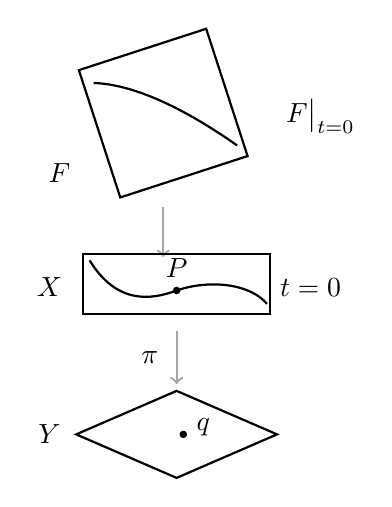
\begin{tikzpicture}[scale=0.85, line width=0.8pt]
  \begin{scope}[rotate around={18:(1.7,4.6)}]
    \draw (0.7,3.6) rectangle (2.7,5.6);
    \draw (0.85,5.35) .. controls (1.4,5.15) and (2.0,4.6) .. (2.6,3.8);
  \end{scope}
  \node at (0.15,3.7) {$\mathscr{F}$};
  \node at (4.05,4.55) {$\mathscr{F}\bigr|_{t=0}$};
  \draw[gray!70,->] (1.7,3.2) -- (1.7,2.45);
  \draw (0.5,1.6) rectangle (3.3,2.5);
  \draw (0.6,2.4) .. controls (1.0,1.75) and (1.5,1.8) .. (1.9,1.95)
        .. controls (2.4,2.12) and (3.0,2.05) .. (3.25,1.75);
  \fill (1.9,1.95) circle (1.6pt);
  \node at (1.9,2.28) {$P$};
  \node at (0.0,2.0) {$\mathscr{X}$};
  \node at (3.9,2.0) {$t=0$};
  \draw[gray!70,->] (1.9,1.35) -- (1.9,0.55);
  \node at (1.5,0.95) {$\pi$};
  \draw (1.9,0.45) -- (3.4,-0.2) -- (1.9,-0.85) -- (0.4,-0.2) -- cycle;
  \fill (2.0,-0.2) circle (1.6pt);
  \node at (2.3,-0.1) {$q$};
  \node at (0.0,-0.2) {$\mathscr{Y}$};
\end{tikzpicture}
\caption{平坦性在源上的（充分的）\trSlicing{}判别法，\mbox{定理~24.6.9}。（依原书手绘图重绘。）}\label{fig:slicing-source-criterion}
\end{figure}

\emph{证明。}\quad 我们有 $A$-\trModule{}（从而也是 $B$-\trModule）的一个\trExactSequence
\[
M \xrightarrow{\ \times t\ } M \longrightarrow M/tM \longrightarrow 0.
\]
把它延拓成 $B$-\trModule{}的一个平坦分解（例如，用自由的 $B$-\trModule{}向左搭出来）：
\[
\tag{24.6.9.1}\label{eq:slicing-source-resolution}
\cdots \longrightarrow M \xrightarrow{\ \times t\ } M \longrightarrow M/tM \longrightarrow 0.
\]
我们可以用任何平坦分解来计算 $\mathrm{Tor}^B_1(M/tM,B/\mathfrak{n})$（\mbox{练习~23.3.D}）。\footnote{译注：原书此处与下文两处均作「$\mathrm{Tor}^B_1(B/tM,B/\mathfrak{n})$」，当为「$\mathrm{Tor}^B_1(M/tM,B/\mathfrak{n})$」之误——\eqref{eq:slicing-source-resolution} 所分解的对象是 $M/tM$，而非「$B/tM$」，径改。——译者注}于是我们使用 \eqref{eq:slicing-source-resolution}。把 $\otimes_B B/\mathfrak{n}$ 作用到 \eqref{eq:slicing-source-resolution} 上，并截去最右一项，便得到这样的\trComplexN，其上同调将给出 $\mathrm{Tor}^B_1(M/tM,B/\mathfrak{n})$：
\[
\cdots \longrightarrow M/\mathfrak{n} \xrightarrow{\ \times t\ } M/\mathfrak{n} \longrightarrow 0.
\]
但由假设，$\times t\colon M/\mathfrak{n}\to M/\mathfrak{n}$ 的\trKernel{}为零，故第一步处的上同调为零，从而我们有 $\mathrm{Tor}^B_1(M/tM,B/\mathfrak{n})=0$。再由平坦性的局部判别法（\mbox{定理~24.6.1}），$M/tM$\footnote{译注：原书此处作「$M/tN$」，当为「$M/tM$」之误，径改。——译者注}在 $B$ 上平坦，此即所欲证。\hfill$\square$

\textbf{24.6.10.}\ \extrahard\ \emph{相对有效\trCartier{}除子。}\quad \mbox{定理~24.6.9} 有一个直接的几何解读：「设 $\pi\colon X\to Y$ 是\trNoether{}概形之间的一个\trMorphism，$\mathscr{F}$ 是 $X$ 上的一个\trCoherentSheaf，而 $Z\hookrightarrow X$ 是一个局部主子概形……」。在 $\mathscr{F}=\OO_X$ 的特殊情形，这就引出了\textbf{相对有效\trCartier{}除子}（relative effective Cartier divisor）的概念：$X$ 的一个局部主子概形，它在 $\pi$ 的一切纤维上都是\trEffectiveCartierDivisor。\mbox{定理~24.6.9} 蕴含：若 $\pi$ 平坦，则任何相对有效\trCartier{}除子也是平坦的。（一个重要应用见\mbox{练习~25.3.H}。）

\textbf{24.6.11. 在域上，正则嵌入是仿射空间中诸坐标轴的局部平坦覆盖。}

\textbf{24.6.B.（有用的练习）}\quad 设 $(A,\mathfrak{m})$ 是一个\trNoether{}局部环，其中 $A$ 包含一个域 $k$（即 $A$ 是一个 $k$-\trAlgebra）。设 $f_1,\dots,f_n\in\mathfrak{m}$。这 $n$ 个 $\Spec A$ 上的函数确定一个\trMorphism{} $\pi\colon\Spec A\to\mathbb{A}^n_k$。证明：$\pi$ 平坦，当且仅当 $f_1,\dots,f_n$ 构成一个\trRegularSequence。更一般地，若 $M$ 是一个有限生成的 $A$-\trModule，证明：$M$ 在 $\mathbb{A}^n_k$ 上平坦，当且仅当 $f_1,\dots,f_n$ 构成一个 $M$-\trRegularSequence。提示：平坦性在靶上的\trSlicing{}判别法，\mbox{定理~24.6.6}。

\mbox{练习~24.6.B} 使许多高深的事实出人意料地变得容易（只要我们是在域 $k$ 上工作）。

\textbf{24.6.C.（练习）}\quad 用\mbox{练习~24.6.B} 给\mbox{定理~9.5.6} 一个直接的证明：$\mathfrak{m}$ 中的 $M$-\trRegularSequence{}在任意重排之下仍是正则的，只要 $A$ 是某个 $k$-\trAlgebra。（「\trMixedCharacteristic」的情形未被覆盖。）我们原来的证明明显更难（尽管更一般）。

\textbf{24.6.D.（练习）}\quad 用\mbox{练习~24.6.B} 重证：\trNoether{} $k$-\trScheme{}中余维数为 $r$ 的\trRegularEmbedding，其（余）正规层是秩 $r$ 的\trLocallyFreeSheaf（\mbox{命题~21.2.16}(b) 的 $k$-\trScheme{}版本）。

\textbf{24.6.E.（练习，参看\mbox{练习~24.1.O}）}\quad 用\mbox{练习~24.6.B} 重证：若 $\mathscr{I}$ 是\trNoether{} $k$-\trScheme{}中余维数为 $r$ 的\trRegularEmbedding{}的理想层，则自然映射 $\Sym^n(\mathscr{I}/\mathscr{I}^2)\to\mathscr{I}^n/\mathscr{I}^{n+1}$ 是\trIsomorphism（\mbox{推论~22.3.9} 的 $k$-\trScheme{}版本）。

\textbf{24.6.F.}\ \extrahard\ \textbf{（练习）}\quad 本练习要用到\mbox{练习~24.4.A}。设 $(A,\mathfrak{m})$ 是一个含域 $k$ 的\trNoether{}局部环，$f_1,\dots,f_r$ 是 $\mathfrak{m}$ 中的一个\trRegularSequence，而 $s$ 把 $E=A^{\oplus r}$ 的第 $i$ 个基元送到 $f_i$。用\mbox{练习~24.6.B} 证明：Koszul 复形 $K_\bullet(s)$（\S24.4.1）正合，唯独在最后一项例外，那里的上同调是 $A/(f_1,\dots,f_r)$。（更一般的陈述见\mbox{练习~24.4.C}。）

\textbf{24.6.12.}\ \extrahard\ \textbf{\trFiber{}平坦性。}\quad 我们以一条可能非常有用的平坦性判别法来收尾，但全书余下的部分并不需要它。它适用于如下由局部\trNoether{}概形组成的交换图，并且其中 $\mathscr{F}$ 是 $X$ 上的一个\trCoherentSheaf：
\[
\begin{tikzcd}[row sep=2.2em, column sep=3.6em]
X \ar[rr, "\pi"] \ar[dr, "\tau"'] & & Y \ar[dl, "\rho"] \\
& Z &
\end{tikzcd}
\]
对每一点 $r\in Z$，令 $\pi_r\colon X_r\to Y_r$ 为 $\pi$ 的基变换。

\textbf{24.6.13. \trFiber{}平坦性定理，版本一。}\ ——\ \emph{设 $\mathscr{F}$ 在 $Z$ 上平坦，且对每一点 $r\in Z$，$\mathscr{F}|_{X_r}$ 在 $Y_r$ 上平坦。则 $\mathscr{F}$ 在 $Y$ 上平坦。}

\textbf{24.6.G.（练习）}\quad 证明：要证\mbox{定理~24.6.13}，只须证明下面这条。

\textbf{24.6.14. \trFiber{}平坦性定理，交换代数版本一。}\ ——\ \emph{设}
\begin{equation*}
\tag{24.6.14.1}\label{eq:fibral-flatness-diagram}
\begin{tikzcd}[row sep=2.4em, column sep=3.4em]
(A,\mathfrak{m}) & & (B,\mathfrak{n}) \ar[ll] \\
& (R,\mathfrak{r}) \ar[ul] \ar[ur]
\end{tikzcd}
\end{equation*}
\emph{是\trNoether{}局部环的一个交换图（照例把极大理想送到极大理想），而 $M$ 是一个有限生成的 $A$-\trModule。设 $M$ 在 $R$ 上平坦，且 $M/\mathfrak{r}M$ 在 $B/\mathfrak{r}B$ 上平坦。则 $M$ 在 $B$ 上平坦。}

\emph{证明。}\quad 我们将使用\mbox{引理~24.6.7}。我们希望证明 $\mathrm{Tor}^B_1(M,B/\mathfrak{n})=0$（以便援引平坦性的局部判别法，\mbox{定理~24.6.1}）；又已知 $M/\mathfrak{r}M$ 在 $B/\mathfrak{r}B$ 上平坦，因此我们希望对模 $M$、环 $B$、理想 $J=\mathfrak{n}$ 与 $I=\mathfrak{r}B$ 应用\mbox{引理~24.6.7}。\mbox{引理~24.6.7} 尚待检验的假设只剩：$\mathrm{Tor}^B_1(M,B/\mathfrak{r}B)=0$。

把右正合函子 $\cdot\otimes_B M$ 作用到 $B$-\trModule{}的满态射 $\mathfrak{r}\otimes_R B\twoheadrightarrow\mathfrak{r}B$ 上，便得到一个满态射
\[
\alpha\colon \mathfrak{r}\otimes_R M=\mathfrak{r}\otimes_R B\otimes_B M \twoheadrightarrow (\mathfrak{r}B)\otimes_B M.
\]
考虑 $B$-\trModule{}映射的复合 $\gamma$：
\[
\mathfrak{r}\otimes_R M \xrightarrow{\ \alpha\ } (\mathfrak{r}B)\otimes_B M \xrightarrow{\ \beta\ } M.
\]
现在 $\alpha$ 是满射，而复合 $\beta\circ\alpha$ 是\trInjectiveMap（把 $\cdot\otimes_R M$ 作用到 $0\to\mathfrak{r}\to R$ 上，并利用 $M$ 在 $R$ 上平坦）。于是 $\alpha$ 必为\trInjectiveMap，从而是\trIsomorphism，进而 $\beta$ 必为\trInjectiveMap。

接下来，把 $M\otimes_B\cdot$ 作用到短正合列
\[
0 \longrightarrow \mathfrak{r}B \longrightarrow B \longrightarrow B/\mathfrak{r}B \longrightarrow 0
\]
上。由于 $B$ 在 $B$ 上平坦，$\mathrm{Tor}^B_1(M,B)=0$，于是我们有正合列
\[
\begin{tikzcd}[row sep=2em, column sep=1.9em]
0=\mathrm{Tor}^B_1(M,B) \ar[r] & \mathrm{Tor}^B_1(M,B/\mathfrak{r}B) \ar[dl] & \\
M\otimes_B\mathfrak{r}B \ar[r, "\beta"] & M\otimes_B B \ar[r] & M\otimes_B B/\mathfrak{r}B \ar[r] & 0.
\end{tikzcd}
\]
由 $\beta$ 的\trInjectiveMap{}性得 $\mathrm{Tor}^B_1(M,B/\mathfrak{r}B)=0$，此即所欲证。\footnote{译注：原书此处作「$\mathrm{Tor}^R_1(M,B/\mathfrak{r}B)$」，其上标当为 $B$（所证者即 $\mathrm{Tor}^B_1$ 的消失），径改。——译者注}\hfill$\square$

\mbox{定理~24.6.14} 可以推广为下面这条（它同样可以引出与\mbox{定理~24.6.13} 类似的几何陈述）。

\textbf{24.6.15. \trFiber{}平坦性定理，交换代数版本二。}\ ——\ \emph{设 \eqref{eq:fibral-flatness-diagram} 是\trNoether{}局部环的一个交换图，而 $M$ 是一个\textbf{非零}的有限生成 $A$-\trModule。则 (a) 成立当且仅当 (b) 成立。}
\begin{itemize}
\item[(a)]\emph{(i) $M$ 在 $R$ 上平坦，且 (ii) $M/\mathfrak{r}M$ 在 $B/\mathfrak{r}B$ 上平坦。}
\item[(b)]\emph{(i) $M$ 在 $B$ 上平坦，且 (ii) $B$ 在 $R$ 上平坦。}
\end{itemize}

\textbf{24.6.H.（容易练习）}\quad 证明：(b) 蕴含 (a)。

\emph{证明。}\quad 结论的大部分已在\mbox{定理~24.6.14} 与\mbox{练习~24.6.H} 中证得。剩下的只须证明：(a)(i)、(a)(ii) 与 (b)(i) 蕴含 (b)(ii)。

\textbf{24.6.I.（练习）}\quad 证明：(a)(i)、(a)(ii) 与 (b)(i) 蕴含 $M$ 在 $B$ 上忠实平坦。

现在我们直接证明 $B$ 在 $R$ 上平坦。设 $N_\bullet$ 是 $R$-\trModule{}的一个\trExactSequence。我们希望证明 $B\otimes_R N_\bullet$ 正合。而由 (a)(i)，$M\otimes_R N_\bullet$ 正合，并且 $M\otimes_R N_\bullet=M\otimes_B(B\otimes_R N_\bullet)$ 正合。由于 $M$ 在 $B$ 上忠实平坦，便知 $B\otimes_R N_\bullet$ 正合，此即所欲证。\hfill$\square$


